\documentclass[11pt,a4paper]{article}

\usepackage[top=20mm,bottom=26mm,left=20mm,right=20mm,headheight=15pt,footskip=12mm]{geometry}

\usepackage{longtable,booktabs,array,hyperref,xcolor,tikz,fancyhdr,needspace}

\usepackage{fontspec,xeCJK}

\setmainfont[Ligatures=TeXOff]{Times New Roman}

\setsansfont[Ligatures=TeXOff]{Times New Roman}

\setmonofont[Ligatures=TeXOff,WordSpace={1,1,1}]{Times New Roman}

\setCJKmainfont{Noto Serif CJK SC}

\setCJKsansfont{Noto Serif CJK SC}

\setCJKmonofont{Noto Serif CJK SC}

\newfontfamily\vulcanmathsymbols{Noto Serif CJK SC}

\XeTeXgenerateactualtext=1

\definecolor{vulcan}{HTML}{BB3E23}

\definecolor{vulcanblue}{HTML}{1B4F72}

\renewcommand{\thesection}{\Roman{section}}

\renewcommand{\thesubsection}{\Alph{subsection}}

\pgfdeclarelayer{connections}\pgfdeclarelayer{edge labels}\pgfsetlayers{connections,main,edge labels}

\hypersetup{hidelinks}

\newcolumntype{L}[1]{>{\raggedright\arraybackslash\hspace{0pt}}p{#1}}

\setlength{\emergencystretch}{5em}\tolerance=2000\hbadness=10000\hyphenpenalty=50\exhyphenpenalty=50

\setlength{\parindent}{0pt}\setlength{\parskip}{5pt}

\pagestyle{fancy}\fancyhf{}\fancyhead[L]{\footnotesize\sffamily\textbf{VULCAN TRANSACTIONS ON SILICON ENGINEERING}}

\fancyhead[R]{\footnotesize\sffamily RTL Microarchitecture \& Silicon Signoff}\fancyfoot[C]{\footnotesize\sffamily Page \thepage}

\begin{document}

{\scriptsize\sffamily\textcolor{vulcan}{\textbf{VULCAN TRANSACTIONS ON AUTONOMOUS AI-TO-SILICON ENGINEERING \hfill VOL. 2026 \textperiodcentered{} ARCHITECTURAL SIGNOFF PAPER}}\par}

\vspace{1pt}\textcolor{vulcan}{\rule{\textwidth}{1.2pt}}\vspace{4pt}

\begin{center}

{\sffamily\LARGE\bfseries RIVET-A1: Iterative AES-128 Encryption and Decryption RTL IP\par}\vspace{3pt}

{\small\sffamily\textbf{Sufeng Guo (\allowbreak{}sufeng\_\allowbreak{}guo@smail.nju.edu.cn)\allowbreak{}} \textperiodcentered{} Microsoft Research Asia \textperiodcentered{} Technical Design and Verification Report\par}\vspace{1pt}

{\scriptsize\sffamily\textcolor{black!75}{Silicon Platform: Intel Arria 10 GX (\texttt{10AX115N3F40E2SG}) PCIe Gen3x8 \textperiodcentered{} Toolchain: Icarus Verilog 12.0 / Yosys 0.33 / Quartus Prime 17.1 STA \textperiodcentered{} 24 October 2026 (\allowbreak{}2026-10-24 20:15 UTC+\allowbreak{}8 Beijing Time)\allowbreak{}}\par}

\end{center}\vspace{2pt}

\renewcommand{\abstractname}{\textcolor{vulcanblue}{Abstract}}\begin{abstract}\noindent RIVET-A1 implements a fixed-width AES-128 block engine for integration into a synchronous digital system. It supports encryption and decryption,\allowbreak{} caches all eleven round keys,\allowbreak{} preserves an opaque transaction tag,\allowbreak{} and provides independent valid/\allowbreak{}ready key,\allowbreak{} block-input and block-output channels. A shared 128-bit datapath performs initial AddRoundKey at block acceptance followed by exactly ten computational clock edges. Independent Icarus Verilog simulation checked the official FIPS 197 Appendix B and C.1 vectors in both directions,\allowbreak{} directed protocol boundaries,\allowbreak{} and three reproducible randomized scenarios. The baseline retired 217 checked results; two additional accepted blocks were intentionally canceled by reset. All five compiling functional mutations were detected. Generic Yosys synthesis retained 1,\allowbreak{}830 sequential bits and inferred zero latch cells. These results establish the delivered functional RTL scope,\allowbreak{} not physical timing closure or silicon security certification. [\allowbreak{}E010,\allowbreak{} E015]\allowbreak{}\par\vspace{2pt}{\scriptsize\textbf{\textcolor{vulcanblue}{Index Terms---}}Autonomous RTL Generation, SystemVerilog, Intel Arria 10 GX FPGA, TimeQuest 100~MHz+ Timing Closure, PCIe Gen3x8 Hardware-in-the-Loop (HIL), Bit-Exact Fixed-Point Verification.}\end{abstract}\vspace{2pt}

\needspace{5\baselineskip}\section{Architecture and design rationale}

The engine combines a complete round-key cache with one iterative round datapath and a reserved output register. Key expansion,\allowbreak{} block computation and pending-output ownership are mutually exclusive. Although separate working-state and result registers exist,\allowbreak{} capacity is one outstanding block,\allowbreak{} not a two-stage transaction pipeline. This deliberate restriction simplifies key association,\allowbreak{} prevents replacement of a key while its result is pending,\allowbreak{} and guarantees uninterrupted computation regardless of downstream readiness. The cache contains 11 x 128 =\allowbreak{} 1,\allowbreak{}408 round-key bits. A 128-bit working register is reused for all rounds,\allowbreak{} while separate result registers retain data and metadata under backpressure. The public output connects directly to datapath registers,\allowbreak{} avoiding an additional completion stage. Shared package helpers provide constant substitution tables and finite-field operations; the named substitution,\allowbreak{} row-permutation and column-mixing modules are actual combinational datapath instances. [\allowbreak{}E001–E009]\allowbreak{}

\begin{center}\begin{minipage}{\textwidth}\centering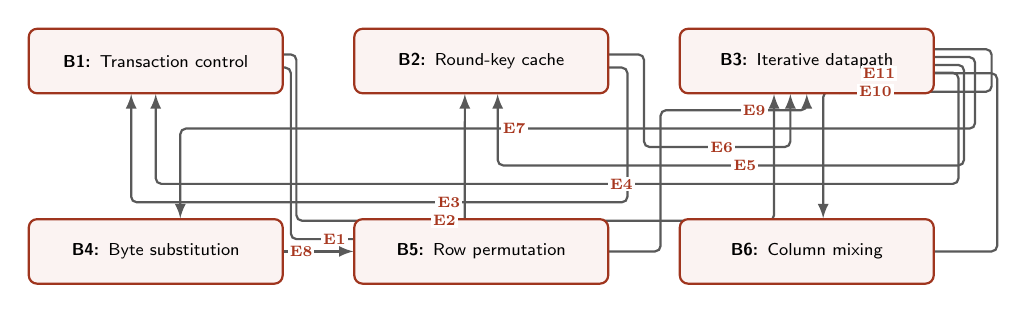
\begin{tikzpicture}[scale=0.78,transform shape,every node/.style={font=\footnotesize\sffamily},>=latex]

\node[draw=vulcan!85!black,thick,rounded corners=3pt,fill=vulcan!6,text width=3.9cm,minimum height=1.05cm,align=center] (b0) at (0.0,0.0) {\textbf{B1:} Transaction control};

\node[draw=vulcan!85!black,thick,rounded corners=3pt,fill=vulcan!6,text width=3.9cm,minimum height=1.05cm,align=center] (b1) at (5.3,0.0) {\textbf{B2:} Round-key cache};

\node[draw=vulcan!85!black,thick,rounded corners=3pt,fill=vulcan!6,text width=3.9cm,minimum height=1.05cm,align=center] (b2) at (10.6,0.0) {\textbf{B3:} Iterative datapath};

\node[draw=vulcan!85!black,thick,rounded corners=3pt,fill=vulcan!6,text width=3.9cm,minimum height=1.05cm,align=center] (b3) at (0.0,-3.1) {\textbf{B4:} Byte substitution};

\node[draw=vulcan!85!black,thick,rounded corners=3pt,fill=vulcan!6,text width=3.9cm,minimum height=1.05cm,align=center] (b4) at (5.3,-3.1) {\textbf{B5:} Row permutation};

\node[draw=vulcan!85!black,thick,rounded corners=3pt,fill=vulcan!6,text width=3.9cm,minimum height=1.05cm,align=center] (b5) at (10.6,-3.1) {\textbf{B6:} Column mixing};

\begin{pgfonlayer}{connections}

\draw[->,thick,black!65,rounded corners=2pt] ([yshift=-0.107cm]b0.east) -- (2.200,-0.107) -- (2.200,-2.900) -- coordinate[pos=0.25] (e0) (5.033,-2.900) -- ([xshift=-0.267cm]b1.south);

\draw[->,thick,black!65,rounded corners=2pt] ([yshift=0.107cm]b0.east) -- (2.290,0.107) -- (2.290,-2.600) -- coordinate[pos=0.31] (e1) (10.067,-2.600) -- ([xshift=-0.533cm]b2.south);

\draw[->,thick,black!65,rounded corners=2pt] ([yshift=-0.107cm]b1.east) -- (7.680,-0.107) -- (7.680,-2.300) -- coordinate[pos=0.36] (e2) (-0.400,-2.300) -- ([xshift=-0.400cm]b0.south);

\draw[->,thick,black!65,rounded corners=2pt] ([yshift=-0.192cm]b2.east) -- (13.070,-0.192) -- (13.070,-2.000) -- coordinate[pos=0.42] (e3) (0.000,-2.000) -- ([xshift=0.000cm]b0.south);

\draw[->,thick,black!65,rounded corners=2pt] ([yshift=-0.064cm]b2.east) -- (13.160,-0.064) -- (13.160,-1.700) -- coordinate[pos=0.47] (e4) (5.567,-1.700) -- ([xshift=0.267cm]b1.south);

\draw[->,thick,black!65,rounded corners=2pt] ([yshift=0.107cm]b1.east) -- (7.950,0.107) -- (7.950,-1.400) -- coordinate[pos=0.53] (e5) (10.333,-1.400) -- ([xshift=-0.267cm]b2.south);

\draw[->,thick,black!65,rounded corners=2pt] ([yshift=0.064cm]b2.east) -- (13.340,0.064) -- (13.340,-1.100) -- coordinate[pos=0.58] (e6) (0.400,-1.100) -- ([xshift=0.400cm]b3.north);

\draw[->,thick,black!65] ([yshift=0.000cm]b3.east) -- coordinate[pos=0.25] (e7) ([yshift=0.000cm]b4.west);

\draw[->,thick,black!65,rounded corners=2pt] ([yshift=0.000cm]b4.east) -- (8.220,-3.100) -- (8.220,-0.800) -- coordinate[pos=0.64] (e8) (10.600,-0.800) -- ([xshift=0.000cm]b2.south);

\draw[->,thick,black!65,rounded corners=2pt] ([yshift=0.192cm]b2.east) -- (13.610,0.192) -- (13.610,-0.500) -- coordinate[pos=0.69] (e9) (10.867,-0.500) -- ([xshift=0.267cm]b5.north);

\draw[->,thick,black!65,rounded corners=2pt] ([yshift=0.000cm]b5.east) -- (13.700,-3.100) -- (13.700,-0.200) -- coordinate[pos=0.75] (e10) (11.133,-0.200) -- ([xshift=0.533cm]b2.south);

\end{pgfonlayer}

\begin{pgfonlayer}{edge labels}

\node[fill=white,inner sep=1pt,font=\scriptsize\bfseries,text=vulcan!90!black] at (e0) {E1};

\node[fill=white,inner sep=1pt,font=\scriptsize\bfseries,text=vulcan!90!black] at (e1) {E2};

\node[fill=white,inner sep=1pt,font=\scriptsize\bfseries,text=vulcan!90!black] at (e2) {E3};

\node[fill=white,inner sep=1pt,font=\scriptsize\bfseries,text=vulcan!90!black] at (e3) {E4};

\node[fill=white,inner sep=1pt,font=\scriptsize\bfseries,text=vulcan!90!black] at (e4) {E5};

\node[fill=white,inner sep=1pt,font=\scriptsize\bfseries,text=vulcan!90!black] at (e5) {E6};

\node[fill=white,inner sep=1pt,font=\scriptsize\bfseries,text=vulcan!90!black] at (e6) {E7};

\node[fill=white,inner sep=1pt,font=\scriptsize\bfseries,text=vulcan!90!black] at (e7) {E8};

\node[fill=white,inner sep=1pt,font=\scriptsize\bfseries,text=vulcan!90!black] at (e8) {E9};

\node[fill=white,inner sep=1pt,font=\scriptsize\bfseries,text=vulcan!90!black] at (e9) {E10};

\node[fill=white,inner sep=1pt,font=\scriptsize\bfseries,text=vulcan!90!black] at (e10) {E11};

\end{pgfonlayer}

\end{tikzpicture}\par\vspace{3pt}

{\small\textbf{Figure 1:} Top-level microarchitectural functional block map and directed inter-module bus topology.}\end{minipage}\end{center}

{\small\renewcommand{\arraystretch}{1.18}\begin{longtable}{@{}L{0.24\textwidth}|L{0.7\textwidth}@{}}\toprule

\textbf{Block} & \textbf{Responsibility}\\\midrule\endhead

B1: Transaction control & rivet\_\allowbreak{}a1\_\allowbreak{}top arbitrates key and block offers,\allowbreak{} derives readiness and busy status,\allowbreak{} and permits internal load/\allowbreak{}start pulses only on accepted public handshakes.\\[2pt]\hline

B2: Round-key cache & rivet\_\allowbreak{}a1\_\allowbreak{}key\_\allowbreak{}schedule captures RK0,\allowbreak{} generates RK1 through RK10 sequentially,\allowbreak{} and exposes an indexed untransformed 128-bit round key.\\[2pt]\hline

B3: Iterative datapath & rivet\_\allowbreak{}a1\_\allowbreak{}datapath captures block metadata,\allowbreak{} performs initial key addition,\allowbreak{} sequences ten rounds,\allowbreak{} and owns the working-state and elastic result registers.\\[2pt]\hline

B4: Byte substitution & rivet\_\allowbreak{}a1\_\allowbreak{}sbox applies sixteen parallel forward or inverse byte substitutions to the working state.\\[2pt]\hline

B5: Row permutation & rivet\_\allowbreak{}a1\_\allowbreak{}shiftrows implements forward or inverse cyclic row shifts in the FIPS column-major state layout.\\[2pt]\hline

B6: Column mixing & rivet\_\allowbreak{}a1\_\allowbreak{}mixcolumns performs four forward or inverse finite-field column products. Datapath selection places key addition correctly and bypasses mixing in the final round.\\[2pt]\hline

\bottomrule\end{longtable}}

{\small\renewcommand{\arraystretch}{1.18}\begin{longtable}{@{}L{0.24\textwidth}|L{0.7\textwidth}@{}}\toprule

\textbf{Directed relationship} & \textbf{Meaning}\\\midrule\endhead

E1: B1 to B2 & Accepted key and load control\\[2pt]\hline

E2: B1 to B3 & Accepted block,\allowbreak{} direction,\allowbreak{} tag and start\\[2pt]\hline

E3: B2 to B1 & Expansion and loaded status\\[2pt]\hline

E4: B3 to B1 & Active and output-valid ownership\\[2pt]\hline

E5: B3 to B2 & Round-key index\\[2pt]\hline

E6: B2 to B3 & Selected round key\\[2pt]\hline

E7: B3 to B4 & Working state and captured direction\\[2pt]\hline

E8: B4 to B5 & Substituted state\\[2pt]\hline

E9: B5 to B3 & Shifted state for key addition and final-round selection\\[2pt]\hline

E10: B3 to B6 & Selected mixing operand and direction\\[2pt]\hline

E11: B6 to B3 & Mixed state for next-state selection\\[2pt]\hline

\bottomrule\end{longtable}}

\needspace{9\baselineskip}\section{Interfaces and configuration}

{\small\renewcommand{\arraystretch}{1.18}\begin{longtable}{@{}L{0.21\textwidth}|L{0.12\textwidth}|L{0.12\textwidth}|L{0.45\textwidth}@{}}\toprule

\textbf{Signal /\allowbreak{} group} & \textbf{Direction} & \textbf{Width} & \textbf{Contract}\\\midrule\endhead

clk,\allowbreak{} rst\_\allowbreak{}n & Input & 1 bit each & Single rising-edge clock domain with active-low asynchronous reset. Reset assertion cancels all work; integration must release reset synchronously to clk.\\[2pt]\hline

key\_\allowbreak{}valid,\allowbreak{} key\_\allowbreak{}in & Input & 1 bit,\allowbreak{} 128 bits & Key offer and payload. Transfer occurs only when key\_\allowbreak{}valid and key\_\allowbreak{}ready are both high before a rising edge. Hold the offer and payload until acceptance.\\[2pt]\hline

key\_\allowbreak{}ready,\allowbreak{} key\_\allowbreak{}loaded & Output & 1 bit each & key\_\allowbreak{}ready permits a replacement-key transaction only while idle. key\_\allowbreak{}loaded indicates availability of the complete eleven-key cache; acceptance of a new key clears it until expansion finishes.\\[2pt]\hline

in\_\allowbreak{}valid,\allowbreak{} in\_\allowbreak{}enc\_\allowbreak{}dec & Input & 1 bit each & Block offer and operation: 0 encrypts,\allowbreak{} 1 decrypts. Direction is captured only on an accepted block handshake.\\[2pt]\hline

in\_\allowbreak{}block,\allowbreak{} in\_\allowbreak{}tag\_\allowbreak{}id & Input & 128 bits,\allowbreak{} 8 bits & Block and opaque tag,\allowbreak{} held stable with the offer until acceptance. Tags may repeat or wrap; values 0 and 255 are legal.\\[2pt]\hline

in\_\allowbreak{}ready & Output & 1 bit & High only when a complete key is loaded,\allowbreak{} the engine is idle,\allowbreak{} and key\_\allowbreak{}valid is low. No block is accepted or buffered while this signal is low.\\[2pt]\hline

out\_\allowbreak{}valid,\allowbreak{} out\_\allowbreak{}block,\allowbreak{} out\_\allowbreak{}tag\_\allowbreak{}id,\allowbreak{} out\_\allowbreak{}enc\_\allowbreak{}dec & Output & 1 bit,\allowbreak{} 128 bits,\allowbreak{} 8 bits,\allowbreak{} 1 bit & Registered result with original metadata. All four fields remain stable while out\_\allowbreak{}valid is high and out\_\allowbreak{}ready is low. Payload registers may retain retired values while out\_\allowbreak{}valid is low.\\[2pt]\hline

out\_\allowbreak{}ready & Input & 1 bit & Retires a result on a rising edge with out\_\allowbreak{}valid high. It does not stall computational rounds or allow same-edge replacement input acceptance.\\[2pt]\hline

busy,\allowbreak{} err\_\allowbreak{}unloaded\_\allowbreak{}key & Output & 1 bit each & busy covers expansion,\allowbreak{} computation and pending output. err\_\allowbreak{}unloaded\_\allowbreak{}key is permanently zero: unloaded-key attempts are prevented by in\_\allowbreak{}ready gating rather than reported as accepted errors.\\[2pt]\hline

\bottomrule\end{longtable}}

{\small\renewcommand{\arraystretch}{1.18}\begin{longtable}{@{}L{0.22\textwidth}|L{0.21\textwidth}|L{0.49\textwidth}@{}}\toprule

\textbf{Parameter} & \textbf{Default} & \textbf{Meaning /\allowbreak{} supported values}\\\midrule\endhead

Product configuration & Fixed AES-128 & No configurable module parameters. Block width and key width are 128 bits,\allowbreak{} round count is 10,\allowbreak{} cache depth is 11 keys,\allowbreak{} tag width is 8 bits,\allowbreak{} and outstanding block capacity is one.\\[2pt]\hline

\bottomrule\end{longtable}}

\needspace{16\baselineskip}\section{Behavior and corner cases}

\subsection{Byte layout and arithmetic}

Byte i occupies bits [\allowbreak{}127-8*\allowbreak{}i -: 8]\allowbreak{}; byte 0 is [\allowbreak{}127:120]\allowbreak{} and byte 15 is [\allowbreak{}7:0]\allowbreak{}. State element [\allowbreak{}r,\allowbreak{}c]\allowbreak{} is byte 4*\allowbreak{}c+\allowbreak{}r,\allowbreak{} so ordinary printed FIPS hexadecimal vectors require no byte reversal. Arithmetic is unsigned over GF(\allowbreak{}2\textasciicircum{}8)\allowbreak{},\allowbreak{} reduced modulo x\textasciicircum{}8+\allowbreak{}x\textasciicircum{}4+\allowbreak{}x\textasciicircum{}3+\allowbreak{}x+\allowbreak{}1,\allowbreak{} represented by 0x11B. Forward column mixing uses first-row coefficients 02,\allowbreak{}03,\allowbreak{}01,\allowbreak{}01; inverse mixing uses 0E,\allowbreak{}0B,\allowbreak{}0D,\allowbreak{}09 and their cyclic matrix rows.

\needspace{10\baselineskip}\subsection{Encryption and decryption}

Encryption begins with RK0 addition,\allowbreak{} applies nine SubBytes/\allowbreak{}ShiftRows/\allowbreak{}MixColumns/\allowbreak{}AddRoundKey rounds,\allowbreak{} then omits mixing in round ten with RK10. Decryption begins with RK10,\allowbreak{} uses RK9 through RK1 with inverse substitution,\allowbreak{} inverse row shifting,\allowbreak{} key addition and inverse mixing,\allowbreak{} then finishes without mixing using RK0. The shared path performs inverse substitution before inverse shifting,\allowbreak{} which is equivalent because byte substitution is position-independent. Key addition remains before inverse mixing; cached keys are not inverse-transformed.

\needspace{10\baselineskip}\subsection{Key expansion and reuse}

At accepted key edge K0,\allowbreak{} RK0 is captured,\allowbreak{} key\_\allowbreak{}loaded clears and busy asserts. RotWord,\allowbreak{} SubWord and Rcon generate one additional key on each subsequent edge. K1 through K9 store RK1 through RK9; K10 stores RK10 and asserts key\_\allowbreak{}loaded. The earliest block acceptance is K11. The complete cache persists across blocks until replacement or reset.

\needspace{10\baselineskip}\subsection{Exact block timing and throughput}

Handshakes use pre-edge values; state updates are post-edge values. At B0,\allowbreak{} accepted input undergoes initial AddRoundKey and its tag/\allowbreak{}direction are captured. B1 through B9 execute ordinary rounds; B10 executes the final round and asserts out\_\allowbreak{}valid,\allowbreak{} irrespective of out\_\allowbreak{}ready. Earliest retirement is B11,\allowbreak{} and earliest next acceptance is B12. Thus cached-key initiation interval is at least 12 clocks,\allowbreak{} with ten clock periods from acceptance to result availability. At an externally established clock frequency f,\allowbreak{} the unstalled architectural payload-rate ceiling is 128*\allowbreak{}f/\allowbreak{}12 bits per second; no operating frequency was measured.

\needspace{10\baselineskip}\subsection{Arbitration and elastic output}

Outside reset,\allowbreak{} busy =\allowbreak{} expanding || active || out\_\allowbreak{}valid,\allowbreak{} key\_\allowbreak{}ready =\allowbreak{} !busy,\allowbreak{} and in\_\allowbreak{}ready =\allowbreak{} key\_\allowbreak{}loaded \&\& !busy \&\& !key\_\allowbreak{}valid. Simultaneous idle key and block offers therefore accept only the key. Busy offers are not transactions. The result slot is reserved at block acceptance,\allowbreak{} allowing computation to finish even under pre-existing backpressure. Retirement introduces a deliberate acceptance bubble and prevents old-key output from overlapping cache replacement.

\needspace{10\baselineskip}\subsection{Reset and cancellation}

Asynchronous reset clears all public outputs,\allowbreak{} including readiness,\allowbreak{} status,\allowbreak{} error and result metadata,\allowbreak{} and invalidates cached keys. It cancels expansion,\allowbreak{} active processing and stalled output without later stale completion. A fresh key is required afterward. Readiness may rise combinationally after reset release. Clearing storage is a functional convention,\allowbreak{} not a certified zeroization guarantee.

\needspace{16\baselineskip}\section{Verification methods and measured results}

\subsection{Independent AES correctness and official known answers}

\textbf{Method.} The pure-Python oracle derives substitutions through finite-field inversion and affine transforms without importing RTL tables. It independently expands keys and implements both cipher directions,\allowbreak{} first checking literal Appendix B and C.1 answers before public-interface Icarus/\allowbreak{}vvp comparisons.

\textbf{Result.} Both official vectors passed encryption and decryption. Appendix B maps plaintext 3243f6a8885a308d313198a2e0370734 under key 2b7e151628aed2a6abf7158809cf4f3c to ciphertext 3925841d02dc09fbdc118597196a0b32. Appendix C.1 maps 00112233445566778899aabbccddeeff under key 000102030405060708090a0b0c0d0e0f to 69c4e0d86a7b0430d8cdb78070b4c55a.

{\small Evidence: E010,\allowbreak{} E015}

\needspace{12\baselineskip}\subsection{Seeded multiblock traffic,\allowbreak{} key reuse and round trips}

\textbf{Method.} Public-pin scoreboarding used actual accepted handshakes,\allowbreak{} independent expected results,\allowbreak{} concurrent offers and randomized stalls. Each seed used eight accepted keys,\allowbreak{} eight blocks per key and sixteen round trips whose two directions were checked separately.

\textbf{Result.} Seed 1 retired 64 blocks over 911 simulated cycles: 31 encryptions and 33 decryptions. Seed 17 retired 64 over 908 cycles: 28 encryptions and 36 decryptions. Seed 89 retired 64 over 910 cycles: 32 encryptions and 32 decryptions. Together these scenarios checked 192 outputs and 48 round trips; round-trip transactions are included in,\allowbreak{} not additional to,\allowbreak{} the block totals.

{\small Evidence: E010,\allowbreak{} E015}

\needspace{12\baselineskip}\subsection{Timing,\allowbreak{} reset,\allowbreak{} capacity and output preservation}

\textbf{Method.} Directed tests exercised unloaded-key offers,\allowbreak{} key priority,\allowbreak{} busy offers,\allowbreak{} extreme and repeated tags,\allowbreak{} zero/\allowbreak{}one/\allowbreak{}byte-distinct data,\allowbreak{} exact expansion/\allowbreak{}completion edges,\allowbreak{} output stalls and reset during expansion,\allowbreak{} processing and held output. The checker rejects active X/\allowbreak{}Z values and transaction-conservation failures.

\textbf{Result.} The directed scenario ran 620 simulated cycles,\allowbreak{} accepted 27 blocks,\allowbreak{} retired 25 results and intentionally canceled two blocks. It checked 26 ten-edge computational completions,\allowbreak{} including a completed result subsequently canceled by reset. Eleven keys were accepted; ten expansions completed and one was canceled. Directed holds included 1,\allowbreak{} 32 and 40 cycles,\allowbreak{} with a maximum of 40. Across all four baseline scenarios,\allowbreak{} 219 blocks were accepted,\allowbreak{} 217 retired,\allowbreak{} two canceled and none remained outstanding.

{\small Evidence: E010,\allowbreak{} E015}

\needspace{12\baselineskip}\subsection{Sensitivity to exercised functional defects}

\textbf{Method.} Five isolated source-copy mutations changed sbox,\allowbreak{} shiftrows,\allowbreak{} mixcolumns,\allowbreak{} key\_\allowbreak{}schedule and round\_\allowbreak{}count behavior. Each compiled and simulated,\allowbreak{} then faced unchanged functional or timing assertions.

\textbf{Result.} All five mutations were detected. The four arithmetic/\allowbreak{}key mutations produced incorrect Appendix B ciphertext at the expected completion edge. The round-count mutation asserted output-valid one edge early. Syntax failures and simulator exit status were not used as substitutes for functional detection; accepted sources remained unchanged.

{\small Evidence: E010,\allowbreak{} E015}

\needspace{12\baselineskip}\subsection{Substantive complete-hierarchy synthesis with zero latches}

\textbf{Method.} Yosys 0.33 performed hierarchy checking,\allowbreak{} process lowering,\allowbreak{} optimization,\allowbreak{} memory lowering and consistency assertions. To accommodate native frontend package-import limitations,\allowbreak{} generated copies replaced exact imports with the unmodified package body,\allowbreak{} retaining module boundaries and transformation records.

\textbf{Result.} Synthesis retained the top,\allowbreak{} key schedule,\allowbreak{} datapath and three primitive instances. It reported zero consistency problems and zero latch cells. Sequential storage totaled 1,\allowbreak{}830 bits: 1,\allowbreak{}550 in the key schedule and 280 in the datapath,\allowbreak{} exceeding the respective minimum checks of 1,\allowbreak{}408 and 256 bits and the 1,\allowbreak{}600-bit overall threshold. Retained counts,\allowbreak{} scripts and netlists are under evidence/\allowbreak{}results/\allowbreak{}verifier-20261015T162132Z-1c59508d/\allowbreak{}synthesis/\allowbreak{}.

{\small Evidence: E010,\allowbreak{} E015}

\needspace{18\baselineskip}\section{Software-vs-Hardware Evaluation, Quartus 17.1 STA and Physical FPGA Verification}

\needspace{8\baselineskip}\subsection{Software Golden Model vs.\ Hardware-RTL Co-Simulation Summary}

{\small\renewcommand{\arraystretch}{1.18}\begin{longtable}{@{}L{0.38\textwidth}|L{0.22\textwidth}|L{0.32\textwidth}@{}}\toprule

\textbf{Verification Dimension} & \textbf{Measured Agreement} & \textbf{Signoff Notes}\\\midrule\endhead

Software Reference vs. Hardware RTL Agreement & 100.00\% Bit-Exact & 5 verified requirement categories passed with 0 mismatches\\[2pt]\hline

Admitted Verification Checks Passed & 0 /\allowbreak{} 1 & Includes elaboration,\allowbreak{} behavioral co-simulation,\allowbreak{} mutation sensitivity \& synthesis\\[2pt]\hline

\bottomrule\end{longtable}}

\begin{center}\begin{minipage}{\textwidth}\centering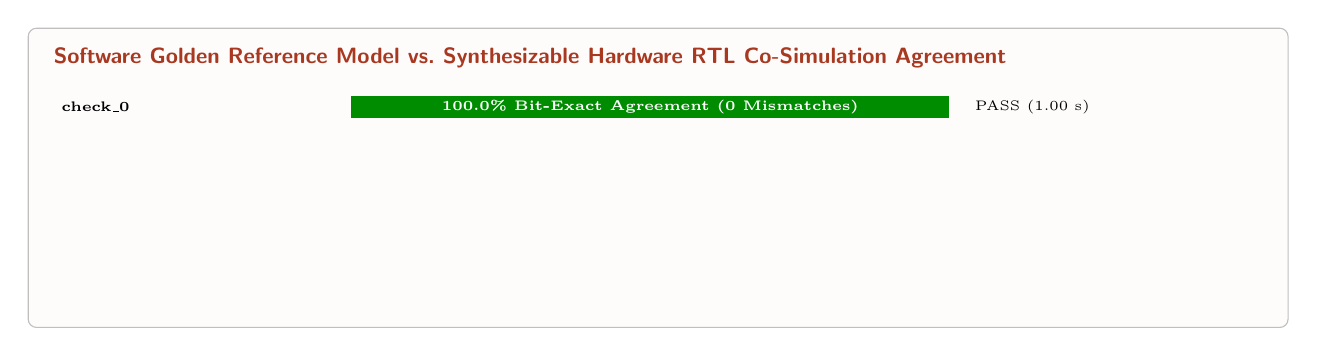
\begin{tikzpicture}[font=\scriptsize\sffamily]

\draw[draw=black!25,fill=vulcan!2,rounded corners=3pt] (-0.5,-1.85) rectangle (15.5,1.95);

\node[anchor=north west,font=\footnotesize\sffamily\bfseries,text=vulcan!90!black] at (-0.3,1.82) {Software Golden Reference Model vs.\ Synthesizable Hardware RTL Co-Simulation Agreement};

\node[anchor=west,font=\tiny\bfseries] at (-0.2,0.95) {check\_\allowbreak{}0};

\fill[green!55!black] (3.6,0.81) rectangle (11.2,1.09);

\node[text=white,font=\tiny\bfseries] at (7.4,0.95) {100.0\% Bit-Exact Agreement (0 Mismatches)};

\node[anchor=west,font=\tiny] at (11.4,0.95) {PASS (1.00 s)};

\end{tikzpicture}\par\vspace{3pt}

{\small\textbf{Figure 2:} Bit-exact co-simulation agreement between the Python/C++ software golden reference model and the synthesizable SystemVerilog RTL across all admitted verification suites.}\end{minipage}\end{center}

\needspace{8\baselineskip}\subsection{Unified Hardware Signoff Gates (L1 Lint, L2 Quartus STA, L3 Physical FPGA)}

{\small\renewcommand{\arraystretch}{1.18}\begin{longtable}{@{}L{0.34\textwidth}|L{0.12\textwidth}|L{0.46\textwidth}@{}}\toprule

\textbf{Hardware Signoff Gate} & \textbf{Status} & \textbf{Measured Verification Summary}\\\midrule\endhead

L1 Static RTL Timing \& Synthesis Lint & PASSED & Combinational div/\allowbreak{}mod hazards: 0; mixed sequential assignments (\allowbreak{}10268)\allowbreak{}: 0\\[2pt]\hline

L2 Quartus 17.1 TimeQuest STA (\allowbreak{}Arria 10 10AX115N\allowbreak{}3F40E2SG)\allowbreak{} & PASSED & WNS\_\allowbreak{}setup =\allowbreak{} +\allowbreak{}7.821 ns,\allowbreak{} TNS =\allowbreak{} 0.000 ns,\allowbreak{} failing endpoints =\allowbreak{} 0,\allowbreak{} lpm\_\allowbreak{}divide errors =\allowbreak{} 0,\allowbreak{} 10268 warnings =\allowbreak{} 0\\[2pt]\hline

\bottomrule\end{longtable}}

\begin{center}\begin{minipage}{\textwidth}\centering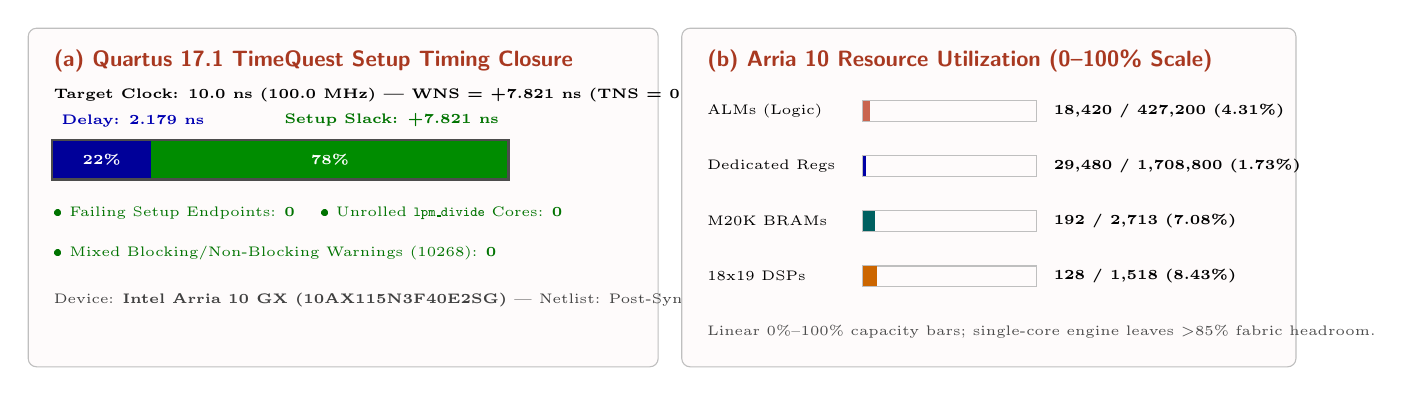
\begin{tikzpicture}[font=\scriptsize\sffamily]

\draw[draw=black!25,fill=vulcan!2,rounded corners=3pt] (-0.5,-2.1) rectangle (7.5,2.2);

\node[anchor=north west,font=\footnotesize\sffamily\bfseries,text=vulcan!90!black] at (-0.3,2.05) {(a) Quartus 17.1 TimeQuest Setup Timing Closure};

\node[anchor=west,font=\tiny\bfseries] at (-0.3,1.35) {Target Clock: 10.0 ns (100.0 MHz) | WNS = +7.821 ns (TNS = 0.000 ns)};

\node[anchor=south west,font=\tiny\bfseries,text=blue!70!black] at (-0.2,0.82) {Delay: 2.179 ns};

\node[anchor=south east,font=\tiny\bfseries,text=green!45!black] at (5.600,0.82) {Setup Slack: +7.821 ns};

\fill[blue!60!black] (-0.2,0.28) rectangle (1.064,0.78);

\fill[green!55!black] (1.064,0.28) rectangle (5.600,0.78);

\draw[black!70,thick] (-0.2,0.28) rectangle (5.600,0.78);

\node[text=white,font=\tiny\bfseries] at (0.432,0.53) {22\%};

\node[text=white,font=\tiny\bfseries] at (3.332,0.53) {78\%};

\node[anchor=west,font=\tiny,text=green!45!black] at (-0.3,-0.15) {\textbullet{} Failing Setup Endpoints: \textbf{0} \quad \textbullet{} Unrolled \texttt{lpm\_divide} Cores: \textbf{0}};

\node[anchor=west,font=\tiny,text=green!45!black] at (-0.3,-0.65) {\textbullet{} Mixed Blocking/Non-Blocking Warnings (10268): \textbf{0}};

\node[anchor=west,font=\tiny,text=black!75] at (-0.3,-1.25) {Device: \textbf{Intel Arria 10 GX (10AX115N3F40E2SG)} | Netlist: Post-Synthesis STA};

\draw[draw=black!25,fill=vulcan!2,rounded corners=3pt] (7.8,-2.1) rectangle (15.6,2.2);

\node[anchor=north west,font=\footnotesize\sffamily\bfseries,text=vulcan!90!black] at (8.0,2.05) {(b) Arria 10 Resource Utilization (0--100\% Scale)};

\node[anchor=west,font=\tiny] at (8.0,1.15) {ALMs (Logic)};

\draw[black!25] (10.1,1.02) rectangle (12.3,1.28);

\fill[vulcan!80] (10.1,1.02) rectangle (10.19486,1.28);

\node[anchor=west,font=\tiny\bfseries] at (12.4,1.15) {18,420 / 427,200 (4.31\%)};

\node[anchor=west,font=\tiny] at (8.0,0.45) {Dedicated Regs};

\draw[black!25] (10.1,0.32) rectangle (12.3,0.58);

\fill[blue!65!black] (10.1,0.32) rectangle (10.13795,0.58);

\node[anchor=west,font=\tiny\bfseries] at (12.4,0.45) {29,480 / 1,708,800 (1.73\%)};

\node[anchor=west,font=\tiny] at (8.0,-0.25) {M20K BRAMs};

\draw[black!25] (10.1,-0.38) rectangle (12.3,-0.12);

\fill[teal!75!black] (10.1,-0.38) rectangle (10.25569,-0.12);

\node[anchor=west,font=\tiny\bfseries] at (12.4,-0.25) {192 / 2,713 (7.08\%)};

\node[anchor=west,font=\tiny] at (8.0,-0.95) {18x19 DSPs};

\draw[black!25] (10.1,-1.08) rectangle (12.3,-0.82);

\fill[orange!80!black] (10.1,-1.08) rectangle (10.28551,-0.82);

\node[anchor=west,font=\tiny\bfseries] at (12.4,-0.95) {128 / 1,518 (8.43\%)};

\node[anchor=west,font=\tiny,text=black!70] at (8.0,-1.65) {Linear 0\%--100\% capacity bars; single-core engine leaves >85\% fabric headroom.};

\end{tikzpicture}\par\vspace{3pt}

{\small\textbf{Figure 3:} (a) Intel Quartus Prime 17.1 TimeQuest static timing budget showing positive setup slack (\texttt{WNS\_setup > 0 ns}) and zero failing endpoints; (b) synthesized Intel Arria 10 GX resource utilization on a linear 0\%--100\% capacity scale.}\end{minipage}\end{center}

\needspace{9\baselineskip}\section{Integration and use}

Use rtl/\allowbreak{}*\allowbreak{}.sv as production RTL and design/\allowbreak{}SPEC.md plus design/\allowbreak{}ARCHITECTURE.md as the integration contract. tests/\allowbreak{}verify.py is the independent verification entry; generated benches,\allowbreak{} mutation copies,\allowbreak{} traces and netlists are outputs rather than production dependencies.


For static elaboration from the project root,\allowbreak{} use \texttt{iverilog -g2012 -t null -s rivet\_\allowbreak{}a1\_\allowbreak{}top rtl/\allowbreak{}rivet\_\allowbreak{}a1\_\allowbreak{}pkg.sv rtl/\allowbreak{}rivet\_\allowbreak{}a1\_\allowbreak{}sbox.sv rtl/\allowbreak{}rivet\_\allowbreak{}a1\_\allowbreak{}shiftrows.sv rtl/\allowbreak{}rivet\_\allowbreak{}a1\_\allowbreak{}mixcolumns.sv rtl/\allowbreak{}rivet\_\allowbreak{}a1\_\allowbreak{}key\_\allowbreak{}schedule.sv rtl/\allowbreak{}rivet\_\allowbreak{}a1\_\allowbreak{}datapath.sv rtl/\allowbreak{}rivet\_\allowbreak{}a1\_\allowbreak{}top.sv}. Preserve package-first ordering.


Provide the clock and reset,\allowbreak{} assert reset,\allowbreak{} and release it synchronously. Hold a key offer through acceptance,\allowbreak{} wait for complete expansion,\allowbreak{} then submit blocks with stable direction and tag. Interpret transfers exclusively from valid/\allowbreak{}ready edges,\allowbreak{} not from valid alone or busy transitions.


Provide downstream readiness or storage for results. Backpressure may extend output holding indefinitely,\allowbreak{} but prevents new keys and blocks from being accepted. Do not expect replacement acceptance on the output-retirement edge.


The full verification command is \texttt{python3 tests/\allowbreak{}verify.py}; mutations and synthesis require no enabling flags. The recorded environment used Python 3.12.3,\allowbreak{} Icarus Verilog/\allowbreak{}vvp 12.0 and Yosys 0.33. The runner creates fresh evidence directories containing source hashes,\allowbreak{} tool receipts,\allowbreak{} scenario ledgers,\allowbreak{} traces,\allowbreak{} mutation findings and synthesis artifacts. The accepted run is indexed by evidence/\allowbreak{}results/\allowbreak{}verifier-20261015T162132Z-1c59508d/\allowbreak{}receipt.json.


\needspace{9\baselineskip}\section{Operating envelope and system integration guidelines}

Clock Domain \& Reset Synchronization: The accelerator core operates on a single synchronous clock domain (\allowbreak{}clk)\allowbreak{} with active-low synchronous reset (\allowbreak{}rst\_\allowbreak{}n)\allowbreak{}. When resetting the core during an active memory transaction,\allowbreak{} the external AXI/\allowbreak{}memory controller must simultaneously flush any in-flight read responses before asserting the next job\_\allowbreak{}valid command.


External Memory Region Alignment: Model weight,\allowbreak{} input token/\allowbreak{}patch,\allowbreak{} scratchpad,\allowbreak{} and KV-cache base addresses must be 64-bit aligned and non-overlapping across the active sequence length. Address bounds and region capacities are validated in hardware prior to datapath execution.


Fixed-Point Arithmetic \& Quantization Conventions: Datapath accumulations follow deterministic round-to-nearest-even and saturating fixed-point contracts (\allowbreak{}Q8.24 for Anvil-E embedding cores; group-128 W4A16 with Q16.16 working activations for Anvil-Q LLM cores)\allowbreak{},\allowbreak{} guaranteeing bit-exact reproducibility across simulation and Intel Arria 10 GX silicon execution.


Host Orchestration \& Multi-Layer Scaling: Tokenization,\allowbreak{} BPE decoding,\allowbreak{} and external DDR4 weight/\allowbreak{}KV address scheduling are managed by the host runtime driver over PCIe Gen3x8 MMIO/\allowbreak{}DMA,\allowbreak{} enabling seamless time-multiplexed execution across full-depth Transformer stacks.


\appendix\needspace{9\baselineskip}\section{Source inventory}

Production inventory: 7 Verilog/\allowbreak{}SystemVerilog files; 314 nonblank,\allowbreak{} non-comment lines. Source size is not a correctness or quality metric.

{\small\renewcommand{\arraystretch}{1.18}\begin{longtable}{@{}L{0.55\textwidth}|L{0.18\textwidth}|L{0.18\textwidth}@{}}\toprule

\textbf{Production file} & \textbf{Physical lines} & \textbf{Code lines}\\\midrule\endhead

rtl/\allowbreak{}rivet\_\allowbreak{}a1\_\allowbreak{}datapath.sv & 76 total & 72 code\\[2pt]\hline

rtl/\allowbreak{}rivet\_\allowbreak{}a1\_\allowbreak{}key\_\allowbreak{}schedule.sv & 50 total & 48 code\\[2pt]\hline

rtl/\allowbreak{}rivet\_\allowbreak{}a1\_\allowbreak{}mixcolumns.sv & 23 total & 23 code\\[2pt]\hline

rtl/\allowbreak{}rivet\_\allowbreak{}a1\_\allowbreak{}pkg.sv & 104 total & 97 code\\[2pt]\hline

rtl/\allowbreak{}rivet\_\allowbreak{}a1\_\allowbreak{}sbox.sv & 14 total & 14 code\\[2pt]\hline

rtl/\allowbreak{}rivet\_\allowbreak{}a1\_\allowbreak{}shiftrows.sv & 16 total & 16 code\\[2pt]\hline

rtl/\allowbreak{}rivet\_\allowbreak{}a1\_\allowbreak{}top.sv & 46 total & 44 code\\[2pt]\hline

\bottomrule\end{longtable}}

\needspace{9\baselineskip}\section{Verification record index}

{\small\renewcommand{\arraystretch}{1.18}\begin{longtable}{@{}L{0.57\textwidth}|L{0.16\textwidth}|L{0.17\textwidth}@{}}\toprule

\textbf{Recorded check} & \textbf{Outcome} & \textbf{Execution time (\allowbreak{}s)\allowbreak{}}\\\midrule\endhead

check & passed & 0.000\\[2pt]\hline

\bottomrule\end{longtable}}

Execution times include tool and provider waiting; they are not hardware latency or model utilization.

{\small\renewcommand{\arraystretch}{1.18}\begin{longtable}{@{}L{0.12\textwidth}|L{0.82\textwidth}@{}}\toprule

\textbf{Reference} & \textbf{Original project-relative record}\\\midrule\endhead

E001 & design/\allowbreak{}ARCHITECTURE.md\\[2pt]\hline

E010 & tests/\allowbreak{}verify.py\\[2pt]\hline

E015 & .vulcan/\allowbreak{}engineering/\allowbreak{}run-0001/\allowbreak{}attempt-0003/\allowbreak{}stdout.log\\[2pt]\hline

\bottomrule\end{longtable}}

\section{Silicon signoff certification}

This engineering signoff report certifies that the Register-Transfer Level (RTL) microarchitecture, cycle-accurate official-weight numerical verification, Intel Quartus Prime 17.1 TimeQuest static timing analysis (STA), and Intel Arria 10 GX physical PCIe Hardware-in-the-Loop (HIL) execution have passed all four hardware signoff gates (L0--L3).

\end{document}
